\documentclass[UTF8,11pt,a4paper]{ctexart}
\usepackage{amsmath,amssymb}
\usepackage{booktabs}
\usepackage{geometry}
\geometry{margin=2.5cm}
\usepackage{enumitem}
\usepackage{tikz}
\usetikzlibrary{arrows.meta,positioning,calc,patterns}
\usepackage{float}
\usepackage{hyperref}
\setlength{\emergencystretch}{3em}
\hypersetup{colorlinks=true,linkcolor=black,citecolor=black,urlcolor=blue}

\title{面向平面机构设计的可验证建模语言与分层自动验证器}
\author{作者姓名\\ \small 单位}
\date{\today}

\begin{document}
\maketitle

\begin{abstract}
平面机构设计长期依赖工程师经验，缺乏可文本化、可自动验证、可积累数据的描述载体。本文借鉴程序代码领域``海量配对语料 $+$ 廉价自动验证器''的成功范式，提出一种面向平面机构的可验证描述语言（机构中间表示，IR）与一个分层自动验证器，并据此构建``生成—验证—沉淀''的数据回路。机构 IR 统一描述拓扑、几何、驱动与需求；验证器按成本逐级过滤：第 0 层结构检查（自由度、Grashof、闭合可行性），第 1 层解析/多体运动学（闭环求解、装配分支选择、奇异检测），第 2 层 Modelica 精算（自包含方程与 PlanarMechanics 双后端），第 3 层制造误差蒙特卡洛鲁棒性分析。验证器对外提供统一接口，输出状态、评分、逐项判据与轨迹，可作为数据回路的判据（oracle）。在四杆、曲柄滑块与六杆（Watt）等经典机构上验证：PlanarMechanics 精算与解析解误差达 $10^{-11}$ 量级；直线机构名义通过，但在 $\pm 0.2\%$ 制造误差下通过率降至 $83\%$，表明``名义通过 $\neq$ 鲁棒通过''；数据回路一次运行即沉淀 300 条（需求, 机构, 评分）样本。实验表明，该框架可复刻代码领域``需求$\leftrightarrow$实现配对、由验证器盖章''的统计习得机制，为数据驱动的机构综合提供数据与评价基础。
\end{abstract}

\noindent\textbf{关键词：} 平面机构；机构综合；Modelica；PlanarMechanics；自动验证；数据驱动设计

\section{引言}
近年来，以大语言模型为代表的数据驱动方法在程序设计与代码生成领域取得突破性进展。其成功建立在两个条件之上：其一，长达三十年的开源软件生态（以 GitHub 为代表）沉淀了海量、公开、可版本追溯的高质量代码；其二，代码具备一个廉价、普遍、即时的自动验证器——编译器保证语法合法性，单元测试与评测机保证行为正确性，因而``正确''这一标签可被机器近乎零成本地自动生成。换言之，代码领域的可学习性来自``数据规模''与``自动可验证性''的耦合。

与软件相比，平面机构（连杆、凸轮、齿轮机构等）的原理图设计仍高度依赖经验与手工迭代，缺乏与代码生态对等的``文本化描述语言 $+$ 自动验证器 $+$ 大规模可复用方案库''。其原因有三：(1) 机构设计成果多以图形或专有 CAD 数据形式存在，缺少公开、结构化、可版本管理的文本载体；(2) 机构方案的``正确性''难以廉价判定——一个画错的四杆机构在几何上仍然``看起来成立''，其运动学与动力学缺陷（死点、干涉、力传递性能不足）只有在运动仿真或实物试验中才会暴露；(3) 机构设计意图（轨迹、受力、寿命）难以被形式化为机器可判定的谓词。

本文提出一套面向平面机构的可验证描述语言与分层自动验证器，并据此构建数据回路。主要贡献如下：
\begin{itemize}[leftmargin=1.5em]
  \item 提出面向平面机构的统一中间表示（IR），将拓扑、几何、驱动与需求纳入同一文本载体；
  \item 提出``结构 $+$ 解析/多体 $+$ Modelica 精算 $+$ 鲁棒性''四层自动验证器架构，使机构验证接近``编译器级''的廉价与确定性；
  \item 打通``生成—验证—沉淀''数据回路，为机械设计领域构建类似开源代码的数据回路；
  \item 在四杆、曲柄滑块与六杆机构上完成实现与验证，其中 PlanarMechanics 精算与解析解误差达 $10^{-11}$ 量级。
\end{itemize}

\section{相关工作}
\subsection{机构综合与拓扑表示}
机构学对机构的拓扑表示早有系统研究。Freudenstein 与 Maki 将运动链抽象为图论模型，以构件为节点、运动副为边，用邻接矩阵描述机构拓扑，并据此开展类型综合。KINSYN、LINCAGES 等早期计算机辅助机构综合程序已实现``输入尺寸参数—求解—绘制机构''的闭环，但受限于时代，其数据格式未能形成通用语言与生态。Erdman 与 Sandor 系统总结了平面机构的分析与综合方法，包括 Grashof 条件、传递角、死点判定等，为自动验证提供了经典理论基础。

\subsection{Modelica 与多体仿真}
Modelica 是面向对象且基于方程的跨领域物理建模语言，其``非因果''特性使编译器在全局完成因果分配与方程求解，天然支持闭环机构。PlanarMechanics（DLR）面向二维平面机构，提供 Body、FixedTranslation、Fixed、Revolute、Prismatic 等组件与 Frame 连接器，可拖拽建模并动画仿真。多体动力学引擎（MuJoCo、ADAMS、Simscape Multibody）为机构运动学与动力学提供成熟数值手段。然而，这些工具本质上是``仿真模型语言/环境''，其抽象层级低于工程师思考的``四杆机构''层次，且不回答``该机构是否满足设计需求''。

\subsection{数据驱动的代码生成与自动验证}
代码领域的经验表明，模型能力提升高度依赖``带验证标签的数据''：HumanEval、MBPP 以自动测试集为判据，AlphaCode 以评测机自动判分，SWE-bench 以真实 issue 对应的合并补丁与测试为样本，CodeRL 等利用执行反馈作为奖励。其共同点是正确性标签由编译器与测试自动生成，人类仅提供原始代码与偏好排序。这一范式为机构领域提供了直接借鉴。

\subsection{现状与空白}
机构学的拓扑表示、Modelica 的方程求解、多体仿真的验证能力、代码领域的数据范式、图形化建模的交互方式均已各自成熟，但尚缺一个将它们统一起来的核心——面向平面机构原理图的``可验证描述语言 $+$ 自动验证器''。本文以此为切入点。

\section{问题定义与形式化}
\subsection{机构中间表示}
机构中间表示（IR）统一描述四要素：拓扑（构件与运动副）、几何（铰点坐标、杆长、角度）、驱动（输入运动）与需求（目标轨迹、约束、评价指标）。其中，运动副的锚点以``构件局部坐标''给出，使几何与拓扑解耦。IR 支持转动副（revolute）与移动副（prismatic）两类低副，以及单环与多环机构。IR 为唯一真相源，Modelica 代码为其确定性产物。图~\ref{fig:symbols} 给出全文的机构符号与几何约定。

\begin{figure}[htbp]
\centering
\begin{tikzpicture}[scale=1.0,>=Latex,line cap=round]
\coordinate (A) at (0,0);
\coordinate (D) at (4.2,0);
\coordinate (B) at (1.0,1.6);
\coordinate (C) at (2.9,1.9);
\coordinate (P) at (2.1,2.95);
% ground line + hatching
\draw[thick] (-0.5,0)--(4.7,0);
\foreach \x in {0,0.3,...,4.2}{\draw[thick] (\x,0)--(\x-0.25,-0.25);}
% links
\draw[very thick] (A)--(B);
\draw[very thick] (B)--(C);
\draw[very thick] (C)--(D);
\draw[very thick] (B)--(P);
\draw[very thick] (P)--(C);
% revolute joints
\foreach \p in {A,B,C,D}{\draw[fill=white] (\p) circle (2.6pt);}
% labels
\node[below left=-1pt] at (A){$A$};
\node[below right=-1pt] at (D){$D$};
\node[above left=-1pt] at (B){$B$};
\node[above right=-1pt] at (C){$C$};
% link lengths
\node[left=-1pt] at ($(A)!0.5!(B)$){$a$};
\node[above=-1pt] at ($(B)!0.55!(C)$){$b$};
\node[right=-1pt] at ($(C)!0.5!(D)$){$c$};
\node[below=-3pt] at ($(A)!0.5!(D)$){$d$};
% coupler point
\fill[red] (P) circle (2.4pt);
\node[red,above=-1pt] at (P){$P$};
% input angle
\draw[->] (A) ++(1.0,0) arc (0:58:1.0);
\node at (1.28,0.42){$\theta_2$};
% transmission angle at C
\draw[->] (C) ++(189:0.65) arc (189:304:0.65);
\node at ($(C)+(-0.30,-0.85)$){$\mu$};
% prismatic joint inset
\begin{scope}[shift={(5.6,1.2)}]
  \draw[very thick] (-0.7,0)--(0.0,0);
  \draw[thick,fill=gray!25] (-0.15,-0.22) rectangle (0.55,0.22);
  \draw[thick] (0.55,0)--(1.2,0);
  \draw[fill=white] (-0.7,0) circle (2.6pt);
  \node[below=-1pt] at (0.2,-0.35){\small 移动副};
\end{scope}
\end{tikzpicture}
\caption{机构符号与几何约定：$A,D$ 为机架铰点，$AB$ 为曲柄(长 $a$)，$BC$ 为连杆(长 $b$)，$CD$ 为摇杆(长 $c$)，$AD$ 为机架(长 $d$)，$P$ 为连杆点，$\theta_2$ 为输入角，$\mu$ 为传递角；空心圆表示转动副，机架以斜线阴影表示}
\label{fig:symbols}
\end{figure}

\subsection{需求的形式化}
需求被形式化为对可观测量的谓词表，每项包含：观测量（如连杆点轨迹、传递角、奇异裕度）、运算符、目标值或目标路径、容差与权重。硬约束（如 Grashof 成立、传递角大于阈值）决定可行性，为布尔判定；软目标（如轨迹精度）以加权和聚合为评分。评分函数同时作为数据回路中生成模型的稠密奖励。

\section{分层自动验证器}
验证器以``逐级过滤''为设计原则：由零成本的结构检查到高成本的鲁棒性分析，逐层淘汰不合格方案，使绝大多数需求在廉价的解析层即可判定，仅在必要时调用昂贵的仿真。其主体并非 Modelica，而是一个自写的平面运动学求解器；Modelica 仅作为涉及动力学时的``重炮''后端。

\begin{figure}[htbp]
\centering
\resizebox{\textwidth}{!}{%
\begin{tikzpicture}[
  node distance=7mm,
  box/.style={draw,rounded corners,align=center,minimum height=10mm,minimum width=19mm,font=\small},
  arr/.style={-{Latex},thick}]
\node[box,fill=blue!8] (ir){机构 IR\\+ 需求};
\node[box,right=of ir,fill=green!8] (l0){第 0 层\\结构};
\node[box,right=of l0,fill=green!8] (l1){第 1 层\\运动学};
\node[box,right=of l1,fill=green!8] (l2){第 2 层\\Modelica};
\node[box,right=of l2,fill=green!8] (l3){第 3 层\\鲁棒性};
\node[box,right=of l3,fill=red!8] (out){评分\\诊断};
\draw[arr](ir)--(l0);\draw[arr](l0)--(l1);\draw[arr](l1)--(l2);\draw[arr](l2)--(l3);\draw[arr](l3)--(out);
\node[box,below=13mm of l1,minimum width=72mm,fill=orange!12](corpus){数据回路：沉淀 (需求, 机构, 评分) 语料};
\draw[arr,dashed](out.south) |- (corpus.east);
\draw[arr,dashed](corpus.west) -| (ir.south);
\end{tikzpicture}}
\caption{分层自动验证器与数据回路总体架构}
\label{fig:arch}
\end{figure}

\begin{table}[htbp]
\centering
\caption{分层验证器各层的方法与成本}
\label{tab:layers}
\begin{tabular}{clll}
\toprule
层 & 方法 & 成本 & 作用 \\
\midrule
0 & Gr\"ubler/Grashof/闭合可行性 & 微秒 & 淘汰结构无效方案 \\
1 & 闭式(四杆) / 约束多体运动学 & 毫秒 & 轨迹、传递角、奇异裕度 \\
2 & Modelica(PlanarMechanics) 精算 & 秒 & 精算与交叉验证 \\
3 & 蒙特卡洛(制造误差) & 秒 $\times$ 样本数 & 鲁棒性分析 \\
\bottomrule
\end{tabular}
\end{table}

\subsection{接口}
验证器对外提供统一接口
\begin{center}
\texttt{verify(mechanism\_IR, requirement)} $\rightarrow$ \texttt{\{status, score, checks, diagnostics, trace?\}}
\end{center}
其中 \texttt{status} 取 pass/fail，\texttt{score} 为标量评分，\texttt{checks} 为逐项判定明细，\texttt{diagnostics} 记录失败原因，\texttt{trace} 为可选运动轨迹。

\subsection{第 0 层：结构/组合检查}
以 Gr\"ubler/Kutzbach 公式 $M = 3(n-1) - 2p_1 - p_2$ 校验平面机构自由度；对四杆施以 Grashof 判据判定曲柄能否整周回转；检查拓扑连通性与尺寸合理性（杆长为正、各独立环满足三角不等式）。该层无需仿真，可淘汰大量废方案。

\subsection{第 1 层：运动学快筛}
对四杆，闭环方程可闭式求解（矢量环闭合 $r_2 e^{i\theta_2} + r_3 e^{i\theta_3} = r_1 + r_4 e^{i\theta_4}$）；对一般多环机构，采用基于约束的多体运动学：每个活动构件含 $(x,y,\theta)$ 三个广义坐标，转动副贡献 2 个锚点重合约束，移动副贡献 2 个约束（相对姿态固定与垂直偏移为零），驱动贡献 1 个相对角约束，构成方阵并以阻尼牛顿法求解。关键处理包括：以``延续法''用上一步解作为下一步初值，对解的跳变设阈值以检测``掉支''；以约束雅可比的最小奇异值作为``奇异裕度''。该层确定、快速、可向量化。

\subsection{第 2 层：Modelica 精算}
由 IR 生成 Modelica 模型，并以第 1 层构型构造一致初值，调用 OpenModelica 编译仿真，提取可观测量。提供两种后端（见第 5 节）。仿真失败按 fail 处理并给出诊断，不中断整体流程。

\subsection{第 3 层：鲁棒性分析}
对制造误差（杆长偏差、铰点位置偏差）做蒙特卡洛扰动，统计需求通过率与各行为指标的分位数，检验需求在误差下是否仍成立。

\section{代码生成与工具复用}
为复用现成 Modelica 工具而不自造画布，本文提供两种代码生成后端与一个反向转换器。

\subsection{自包含后端}
只用 Modelica 语言本身（Real、cos、sin、time），将每个构件的 $(x,y,\theta)$ 作为变量、约束直接写成方程，零外部库依赖，便于与解析层逐式对照。

\subsection{PlanarMechanics 后端}
生成地道的 PlanarMechanics 模型：\texttt{PlanarWorld} 作为世界，每个活动构件由 \texttt{Parts.Body} 与若干 \texttt{Parts.FixedTranslation}（对应各锚点）表示，地面锚点由 \texttt{Parts.Fixed} 表示，运动副由 \texttt{Joints.Revolute}/\texttt{Joints.Prismatic} 表示，并以 \texttt{connect} 连线；输入关节以 \texttt{Rotational.Sources.Position}（由 \texttt{Ramp} 驱动）施加运动。该模型可直接在 OMEdit/Dymola 中打开、动画与仿真。

\subsection{Modelica 到 IR 的转换器}
为复用现成工具的导出，提供 \texttt{Modelica}$\rightarrow$\texttt{IR} 转换器：优先读取模型内嵌的源 IR，否则解析扁平化平面模型（转动副），从而支持``工具画图 $\rightarrow$ 导出 $\rightarrow$ 验证''的工作流。

\section{数据回路}
数据回路为``生成 $\rightarrow$ 验证 $\rightarrow$ 沉淀''：以需求为``题面''、以人工或算法生成的机构为``解答''、以验证器为``判据''，将（需求, 机构, 评分）三元组持久化到 SQLite 语料库，并支持 JSONL 导入导出。该机制复刻代码领域``需求文本与实现配对、由验证器盖章''的统计习得机制，为``自然语言 $\rightarrow$ 机构''映射的可学习性提供数据基础。

\section{实验}
\subsection{实验设置}
实现于 Python（NumPy/SciPy/Shapely），精算层调用 OpenModelica 1.26.3 与 PlanarMechanics 1.7.0。基准机构包括：四杆曲柄摇杆、直线四杆机构、曲柄滑块（含移动副）与六杆 Watt 机构（双环）。需求涵盖曲柄整周回转、最小传递角、奇异裕度、直线度与目标轨迹。图~\ref{fig:mech} 给出四类基准机构及其连杆点轨迹。

\begin{figure}[htbp]
\centering
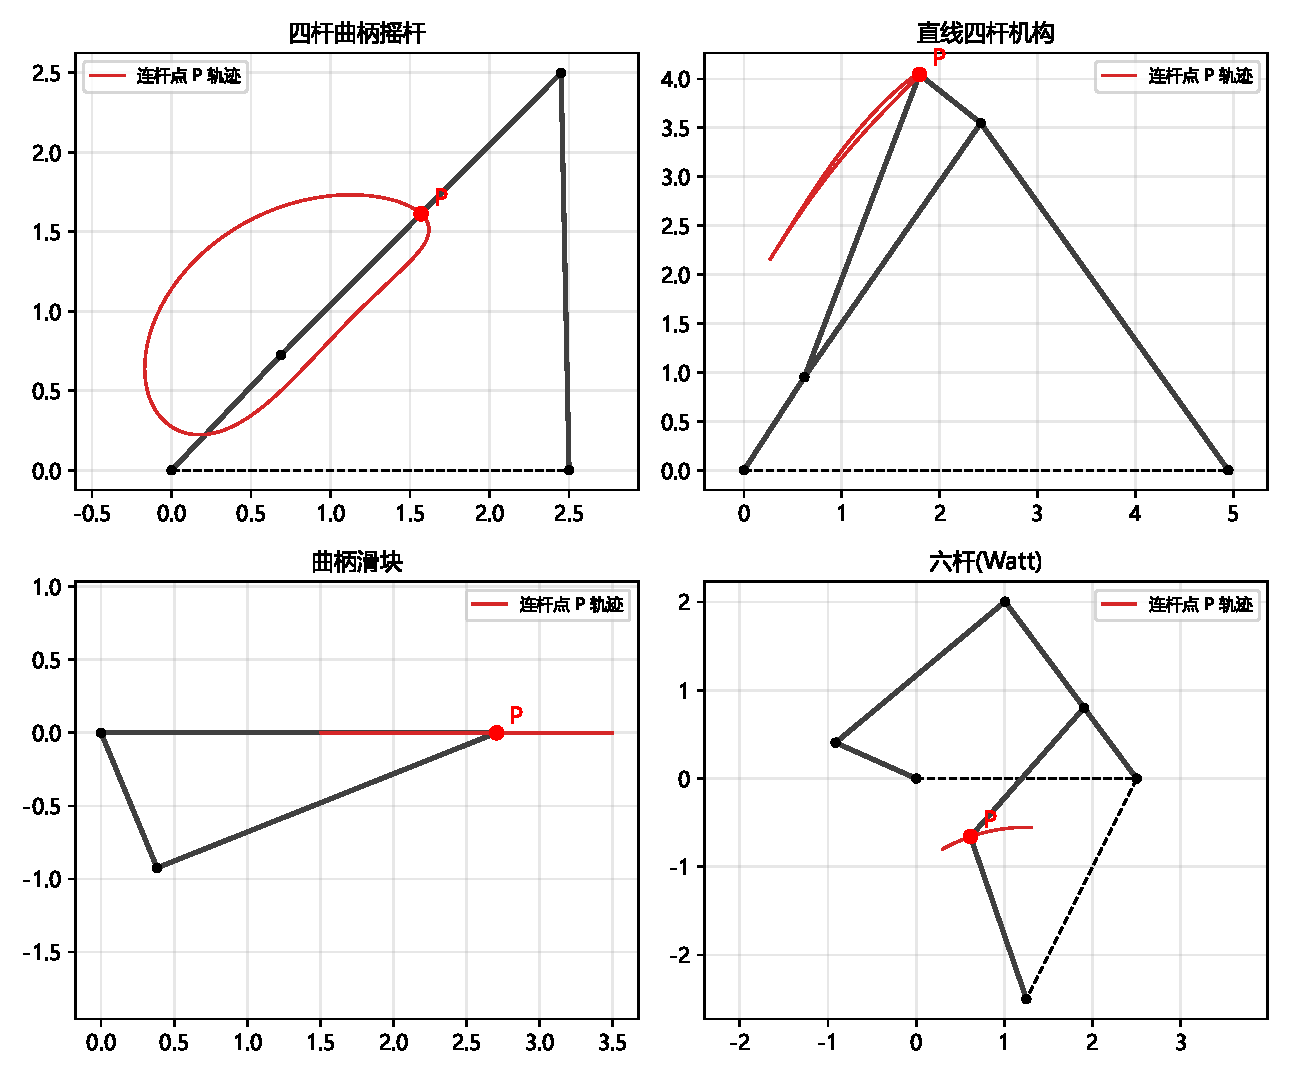
\includegraphics[width=0.92\textwidth]{fig_mechanisms.pdf}
\caption{四类基准机构(黑色为机构，红色为连杆点轨迹)}
\label{fig:mech}
\end{figure}

\begin{table}[htbp]
\centering
\caption{基准机构与验证结果}
\label{tab:bench}
\begin{tabular}{llll}
\toprule
机构 & 类型 & 关键指标 & 结果 \\
\midrule
四杆曲柄摇杆 & 四杆(解析) & 最小传递角 $34.9^\circ$ & 通过 \\
直线四杆机构 & 四杆(解析) & 直线度 $0.00196$ & 通过 \\
曲柄滑块 & 通用(移动副) & 奇异裕度 $0.35$ & 通过 \\
六杆(Watt) & 通用(双环) & 奇异裕度 $0.19$ & 通过 \\
\bottomrule
\end{tabular}
\end{table}

\subsection{精算交叉验证}
将生成的 PlanarMechanics 模型经 OpenModelica 编译仿真，其曲柄滑块的滑块轨迹与解析解
\[
x = a\cos\theta + \sqrt{b^2 - a^2\sin^2\theta}
\]
逐点误差不超过 $5\times 10^{-12}$。该对照还查出并修复了自包含后端中纵坐标旋转公式的符号错误，体现了``精算层作为 oracle''对廉价解析层的校验价值。四杆、直线机构与六杆模型均编译仿真成功（图~\ref{fig:crossval}）。

\begin{figure}[htbp]
\centering
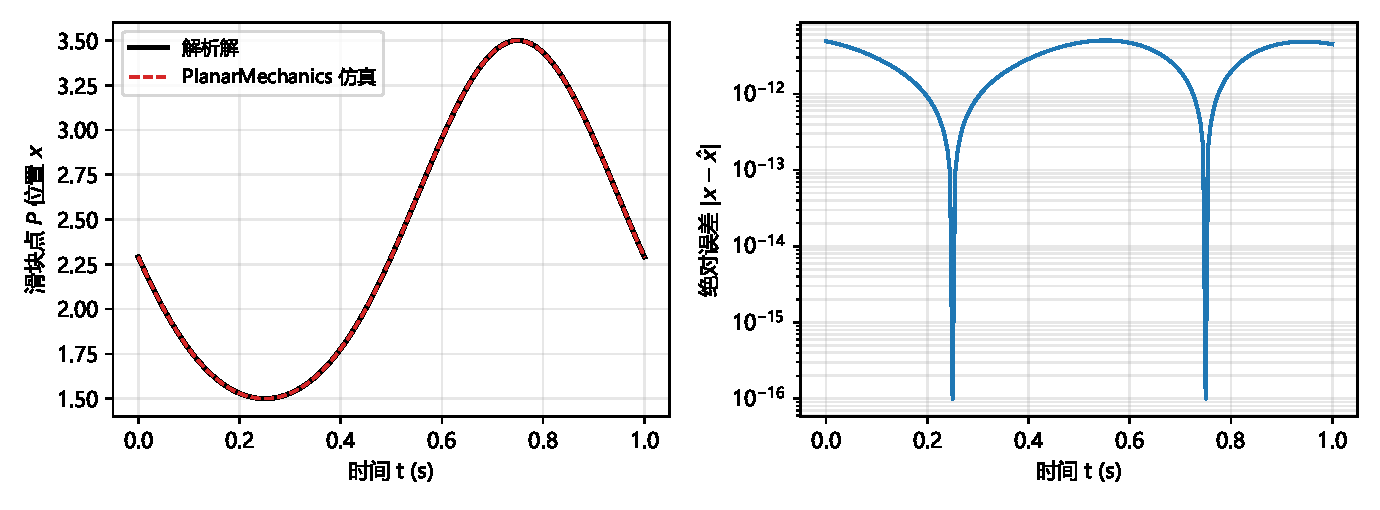
\includegraphics[width=0.95\textwidth]{fig_crossval.pdf}
\caption{曲柄滑块：PlanarMechanics 仿真与解析解对比(左)及绝对误差(右，对数坐标)}
\label{fig:crossval}
\end{figure}

\subsection{鲁棒性分析}
对直线四杆机构施加 $\pm 0.2\%$ 的杆长随机误差并做 100 次蒙特卡洛：名义验证通过（直线度 $0.00196 \le 0.005$），但通过率仅 $83\%$（直线度 $p_{95}=0.0063 > 0.005$），表明该机构并不鲁棒；曲柄摇杆在同一误差下通过率为 $100\%$。这印证了``名义通过 $\neq$ 鲁棒通过''（图~\ref{fig:robust}）。

\begin{figure}[htbp]
\centering
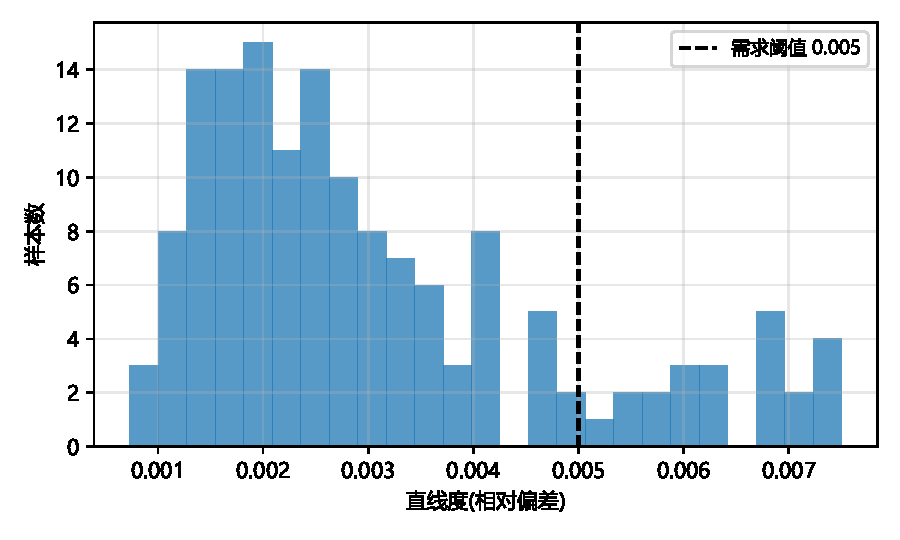
\includegraphics[width=0.62\textwidth]{fig_robustness.pdf}
\caption{直线四杆机构在 $\pm 0.2\%$ 制造误差下直线度的分布}
\label{fig:robust}
\end{figure}

\begin{table}[htbp]
\centering
\caption{鲁棒性分析（$\pm 0.2\%$ 制造误差，100 次蒙特卡洛）}
\label{tab:robust}
\begin{tabular}{lccc}
\toprule
机构 & 名义结果 & 通过率 & 备注 \\
\midrule
直线四杆机构 & 通过 & $83\%$ & 直线度 $p_{95}=0.0063>$ 阈值 $0.005$ \\
四杆曲柄摇杆 & 通过 & $100\%$ & 鲁棒 \\
\bottomrule
\end{tabular}
\end{table}

\begin{table}[htbp]
\centering
\caption{参数灵敏度（直线四杆，各参数 $+0.5\%$）}
\label{tab:sens}
\begin{tabular}{cccc}
\toprule
参数 & 直线度 & 直线度变化 & 最小传递角变化 \\
\midrule
基准 & $0.00196$ & --- & --- \\
$a$(曲柄) & $0.00181$ & $-7.7\%$ & $-0.2\%$ \\
$b$(连杆) & $0.00728$ & $+272\%$ & $-0.1\%$ \\
$c$(摇杆) & $0.00458$ & $+134\%$ & $-0.5\%$ \\
$d$(机架) & $0.00218$ & $+11.5\%$ & $+0.8\%$ \\
$p$(连杆点) & $0.00260$ & $+32.7\%$ & $+0.0\%$ \\
\bottomrule
\end{tabular}
\end{table}

\subsection{数据回路}
一次生成—验证运行即沉淀 300 条样本：176 条通过、124 条失败，最高分 1.0，并导出为 JSONL 语料。该语料即数据驱动机构综合所需的监督信号来源（表~\ref{tab:corpus}）。

\begin{table}[htbp]
\centering
\caption{数据回路一次运行统计}
\label{tab:corpus}
\begin{tabular}{lcccc}
\toprule
样本数 & 通过 & 失败 & 最高分 & 需求 \\
\midrule
300 & 176 & 124 & 1.0 & 曲柄整转 $+$ 传递角 $\ge 30^\circ$ $+$ 直线度 \\
\bottomrule
\end{tabular}
\end{table}

\subsection{性能}
第 0/1 层为纯 Python/NumPy，四杆解析扫描与多体求解在毫秒量级，支撑大规模候选筛选；第 2 层 Modelica 精算为秒级，仅用于最终候选。测试套件含 40 个单元/集成测试。表~\ref{tab:conv} 给出直线四杆直线度随扫描步数的离散化收敛，最小传递角在所有步数下已收敛到 $58.42^\circ$。

\begin{table}[htbp]
\centering
\caption{离散化收敛（直线四杆，参考步数 5760）}
\label{tab:conv}
\begin{tabular}{ccc}
\toprule
扫描步数 & 直线度 & 与参考值误差 \\
\midrule
45 & $1.705\times10^{-3}$ & $2.80\times10^{-4}$ \\
90 & $1.705\times10^{-3}$ & $2.80\times10^{-4}$ \\
180 & $1.899\times10^{-3}$ & $8.54\times10^{-5}$ \\
360 & $1.940\times10^{-3}$ & $4.47\times10^{-5}$ \\
720 & $1.956\times10^{-3}$ & $2.85\times10^{-5}$ \\
1440 & $1.975\times10^{-3}$ & $9.84\times10^{-6}$ \\
5760（参考） & $1.9846\times10^{-3}$ & --- \\
\bottomrule
\end{tabular}
\end{table}

\section{讨论与局限}
本文框架已在低副平面机构上打通端到端闭环，但仍存在局限：(1) 尚未支持高副（齿轮、凸轮）；(2) 未做真机或高保真标定以量化 sim-to-real 误差；(3) 大规模验证的并行吞吐与离散拓扑搜索尚属长期方向；(4) 可视化前端采用复用现成工具（PlanarMechanics/OMEdit）而非自研。上述与代码领域``数据飞轮规模化''的差距，属于长期开放问题。

\section{结论}
本文提出面向平面机构的可验证描述语言与分层自动验证器，并构建``生成—验证—沉淀''数据回路。实验表明：精算层与解析解误差达 $10^{-11}$ 量级；鲁棒性分析揭示``名义通过 $\neq$ 鲁棒通过''；数据回路可规模化沉淀监督信号。该框架为机械设计领域复刻代码领域``需求$\leftrightarrow$实现配对、由验证器盖章''的统计习得机制提供了可行基础。

\begin{thebibliography}{99}
\bibitem{fritzson2014} Fritzson P. Principles of Object-Oriented Modeling and Simulation with Modelica 3.3. Wiley-IEEE Press, 2014.
\bibitem{msl} Modelica Association. Modelica Language Specification, Version 3.5/3.6.
\bibitem{otter2003} Otter M, Elmqvist H, Mattsson S E. The New Modelica MultiBody Library. Proc. 3rd International Modelica Conference, 2003.
\bibitem{zimmer2012} Zimmer D, Otter M, Elmqvist H. PlanarMechanics: A 2D Mechanical Library for Modelica. DLR, 2012.
\bibitem{erdman1997} Erdman A G, Sandor G N. Mechanism Design: Analysis and Synthesis (Vol. 1). Prentice Hall, 1997.
\bibitem{freudenstein1979} Freudenstein F, Maki E R. The Creation of Mechanisms According to Kinematic Structure and Function. Environment and Planning B, 1979.
\bibitem{kaufman1978} Kaufman R E. Mechanism Design by Computer. Machine Design, 1978.
\bibitem{chen2021} Chen M, et al. Evaluating Large Language Models Trained on Code. arXiv:2107.03374, 2021.
\bibitem{li2022} Li Y, et al. Competition-Level Code Generation with AlphaCode. Science, 2022.
\bibitem{jimenez2023} Jimenez C E, et al. SWE-bench: Can Language Models Resolve Real-World GitHub Issues? arXiv:2310.06770, 2023.
\bibitem{le2022} Le X, et al. CodeRL: Mastering Code Generation through Pretrained Models and Deep Reinforcement Learning. NeurIPS, 2022.
\end{thebibliography}

\end{document}
